\documentclass[12pt]{article}

\usepackage[italian]{babel}
\usepackage{graphicx} 
\usepackage{fancyhdr}
\usepackage[a4paper,top=3cm,bottom=3cm,left=3cm,right=3cm]{geometry}
%\usepackage[export]{adjustbox}
%\usepackage{wrapfig}
\usepackage{subcaption}
\usepackage{float}
\usepackage{listings}
\lstset{basicstyle=\ttfamily,
  showstringspaces=false,
  basicstyle=\footnotesize\ttfamily,
  numbers=left,
  stepnumber=1,
  numbersep=10pt,    
  columns=fullflexible,
  frame=single,
  breaklines=true,
  numberstyle=\small
}

\title{Relazioni Internet}
\author{Squadra A\\Gruppo 16}
\date{}

\lhead{
\begin{minipage}[c][2cm][c]{\textwidth}
 \textbf{Laboratori di internet e comunicazioni}
\end{minipage}
}
\rhead{
\includegraphics[width = 2.5cm]{logo_poli.png}}
\renewcommand{\headrulewidth}{0pt}
\setlength{\headheight}{3cm}

\pagestyle{plain}

\begin{document}


\maketitle
\thispagestyle{fancy}


\newpage

\setcounter{page}{1}
\setlength{\headheight}{0cm}

\section{Secondo laboratorio}
In questo laboratorio abbiamo analizzato il funzionamento del protocollo TCP sfruttando il servizio CHARGEN.\\
In particolare abbiamo utilizzato il client telnet per effettuare una richiesta al server CHARGEN, sulla porta associata a tale servizio, usando il comando:
\begin{verbatim}
  telnet [host] [port] #utilizzando la porta 19
\end{verbatim}
Per evitare frammentazione a livello ethernet abbiamo disattivato le opzioni avanzate della scheda di rete con il seguente script
\begin{verbatim}
  #!/bin/bash
  sudo ethtool -K eth0 rx off
  sudo ethtool -K eth0 tx off
  sudo ethtool -K eth0 sg off
  sudo ethtool -K eth0 tso off
  sudo ethtool -K eth0 ufo off
  sudo ethtool -K eth0 gso off
  sudo ethtool -K eth0 gro off
  sudo ethtool -K eth0 lro off
\end{verbatim}
Per generare i grafici relativi alla simulazione sono state catturate le informazioni relative ai pacchetti trasmessi, per poi essere esportate come file di testo, utilizzando wireshark. In seguito tali file sono stati rielaborati utilizzando 2 script in bash.\\
Un ulteriore grafico relativo alla velocità di trasmissione è stato generato utilizzando la funzione \textit{grafici I/O} di wireshark.\\
Le 2 schede di rete sono state impostate in full-duplex a 100Mb/s.
\\\\
\textit{I files utilizzati per la creazione dei grafici si trovano in appendice.}
\\\\
Nel corso della simulazione sono state compiute alcune azioni, di seguito elencate, che permettono di identificare diversi intervalli:
\begin{enumerate}
\item Finestra massimizzata
\item Finestra minimizzata
\item Finestra massimizzata
\item Output bloccato (ctrl+C)
\item Nuovo terminale con secondo telnet e output bloccato (ctrl+C)
\item Command-mode (primo terminale)
\item Ripristino ricezione (primo terminale)
\item Chiusura connessione
\end{enumerate}

\subsection{Analisi lato client}
Il grafico in \textit{figura 1} mostra il campo Ack dei pacchetti TCP inviati dal server al primo terminale aperto.
Ogni Ack avrà un valore incrementato pari al valore del’ultima Ack sommata alla grandezza dell’ultimo pacchetto ricevuto. Infatti l’Ack indica al server quale dovrà essere il prossimo pacchetto ad essere inviato usando i byte trasmessi dal server come “contatori”, in modo da poter evitare eventuali errori di trasmissione.
Dunque le ack possono essere utilizzate come mezzo per sapere quanti dati sono stati ricevuti nel tempo e ottenere un grafico la cui derivata indica la velocità di ricezione del client.

\subsubsection{Intervallo 1-2-3}	
Durante l’intervallo 1 e 2 notiamo che la velocità non subisce variazioni a contrario di quanto si potrebbe pensare. Ciò che potremmo aspettarci è una diminuzione di velocità passando da 1 a 2 per poi tornare al valore iniziale in 3. \\Infatti nella fase 1, dal momento che il terminale avrà dimensione massima, telnet richiederà il massimo numero di caratteri a differenza di quanto farà in 2, dove le dimensioni minori del terminale porteranno a una minor richiesta di caratteri al secondo. Tuttavia ciò che avviene è che la variazione di velocità non è abbastanza significativa da permetterci di osservare differenze sostanziali nel grafico. Possiamo notare nel grafico in \textit{figura 2}, il quale rappresenta l’evoluzione della finestra di ricezione del client nel tempo, come il client continuerà a modificare tale valore, senza mai raggiungere un valore stabile a causa dell'output. Infatti nel momento in cui il client riceverà dati si ritroverà costretto ad accumularli in un buffer a causa della latenza dovuta all'output. Quando il buffer sarà quasi pieno la finestra diminuirà, in modo da richiedere meno dati e permettere al buffer di svuotarsi.\\

\begin{figure}[h]
  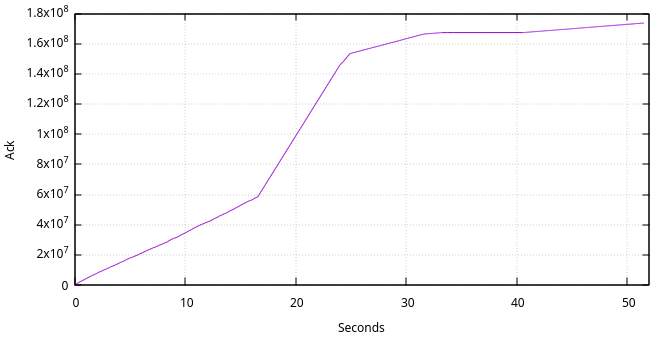
\includegraphics[height=5.5cm]{client_ack_lines.png}
  \centering
  \caption{Ack lato client}
  \label{client_ack}
\end{figure}

\begin{figure}[h]
  \centering	
  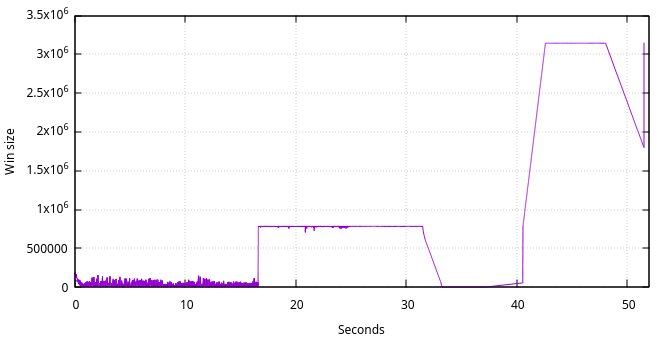
\includegraphics[height=5.5cm]{client_win_lines.png}
  \caption{Win lato client }
  \label{client_ack}
\end{figure}

\begin{figure}[H]
  \centering
  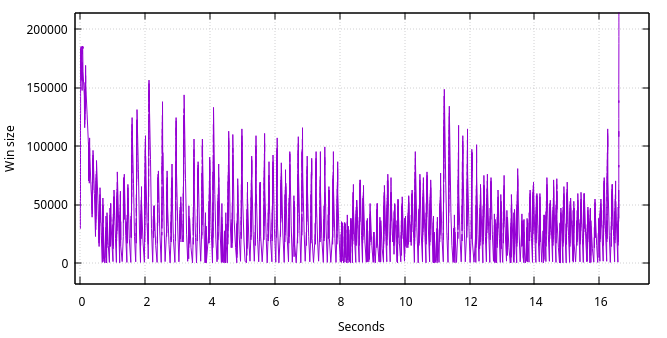
\includegraphics[height=5.5cm]{client_win_lines_zoom.png}
  \caption{Dettaglio \textit{figura 2} }
  \label{client_ack_zoom}
\end{figure}

\subsubsection{intervallo 4}
Durante l'intervallo 4 la pressione di ctrl+C porterà telnet a richiedere il massimo numero di dati da lui ricevibili nell'unità di tempo, senza doverli stampare e evitando di conseguenza rallentamenti dovuti all'output.\\ 
Possiamo notare in \textit{figura 2} come la finestra riesca in questo caso a raggiungere un valore stabile e costante.
Infatti grazie all'assenza dell'output il client non presenterà ritardi e potrà comunicare una finestra più ampia.\\
Notare che ciò si traduce con un'incremento sostanziale della velocità di trasmissione del server.

\subsubsection{Intervallo 5}
Nell’intervallo 5, in cui viene aperta una nuova connessione al server, ci aspettiamo un dimezzamento della velocità data dalla divisione della banda tra i 2 terminali. Tuttavia come possiamo notare in \textit{figura 3}, dove osserviamo la velocità di trasmissione verso i 2 client da parte del server, la banda non viene dimezzata. Possiamo notare che la velocità non viene ridistribuita equamente e che la scarsa velocità del primo client ad essere stato aperto giustifichi la diminuzione della pendenza in \textit{figura 1}.
Notare come in \textit{figura 2} non sia cambiata l'ampiezza della finestra.
Ciò ci porta alla conclusione che il client è in grado di modificare la propria finestra di ricezione a piacimento e di comunicarla, tuttavia non sempre il server potrà soddisfare tale richiesta.\\

\begin{figure}[H]
  \center	
  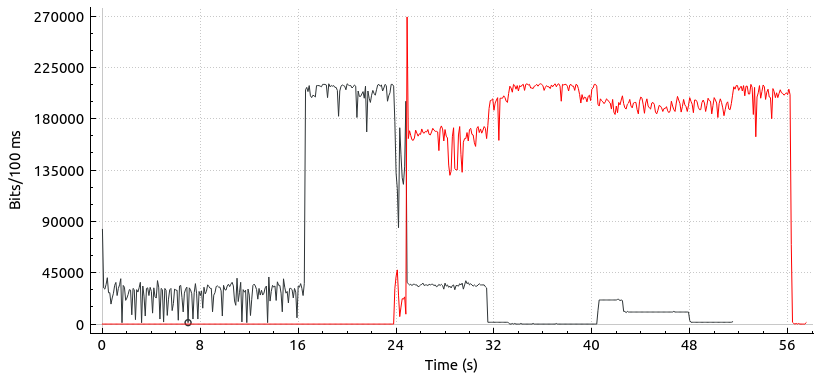
\includegraphics[height=5cm]{client_wireshark_speed.png}
  \caption{Velocità di trasmissione ai 2 client}
  \label{I/O}
\end{figure}

\subsubsection{intervallo 6}
Nell’intervallo 6 la command mode causa un’arresto della trasmissione dei dati, ma non dello scambio di pacchetti. Ciò che si evince è che nonostante la connessione tra i 2 dovrebbe essere interrotta, vi sarà comunque un passaggio di pacchetti, come mostrato in \textit{figura 5}, in cui vengono mostrati i numeri di ACK e SEQ dei pacchetti inviati rispettivamente da client e server (\textit{spiegazione nella sezione 2}) senza interpolazione.\\
Ciò avviene in quanto, una volta ridotta la finestra di ricezione del client (\textit{figura 2}) il server continuerà a inviare pacchetti vuoti, come mostrato dal grafico del payload in \textit{figura 16}, per permettere al client di comunicare la propria finestra e assicurarsi di conseguenza che il client sia ancora in command-mode.\\
Notare anche come la cadenza di tali pacchetti diminuisca gradualmente con il tempo. Il che ci porta ad ipotizzare che la ripresa della trasmissione non sia sincronizzata con la pressione del tasto invio (\textit{vedi sezione 1.3})

\begin{figure}[H]
	\begin{subfigure}[l]{0.5\linewidth}
		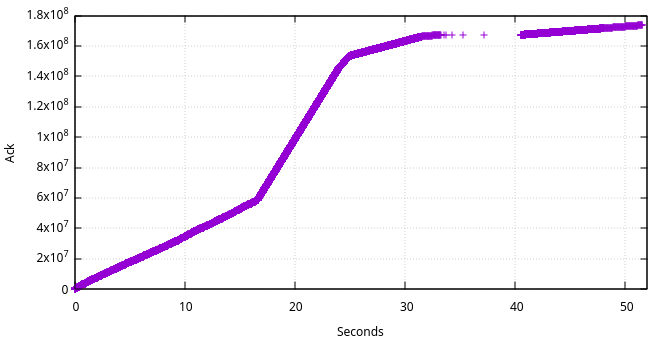
\includegraphics[width=\linewidth]{client_ack_point.png}
		\caption{client)}
	\end{subfigure}	
	\begin{subfigure}[r]{0.5\linewidth}
		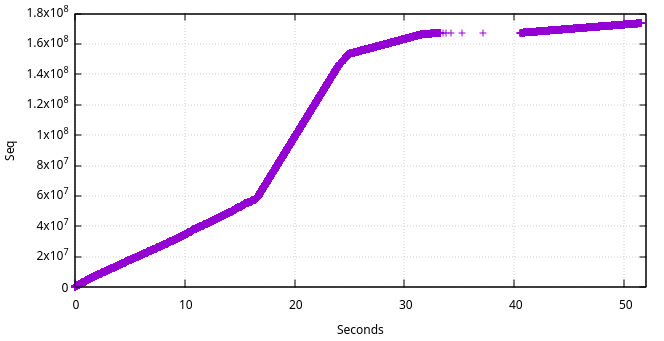
\includegraphics[width=\linewidth]{server_seq_point.png}
		\caption{server}
	\end{subfigure}
	\caption{Grafici dei singoli pacchetti senza interpolazione}
	\label{ack_and_seq_point}
\end{figure}

\subsubsection{intervallo 7-8}
Nell’intervallo 7 viene ripristinato il flusso dei dati uscendo dalla command-mode, per poi chiudere la connessione nell’intervallo 8.\\
Notare che la trasmissione non riprenderà con la stessa velocità (\textit{figura 4}), ma il primo client sarà più lento rispetto all'intervallo 5 e di conseguenza il grafico relativo alle Ack del client presenterà una pendenza inferiore (\textit{figura 1}).
Possiamo notare di nuovo come la finestra di ricezione (che assumerà un valore ancora più alto che in precedenza) sia indipendente dalla velocità che può essere garantita dal server in un determinato momento, dato che a una finestra ampia corrisponde una velocità scarsa.
In fase di chiusura si nota una diminuzione della finestra dovuta alla command-mode e un ultimo picco dovuto alla trasmissione dei pacchetti adibiti alla chiusura della connessione.

\subsection{Considerazioni lato server}
Per quanto riguarda il server possiamo notare lo stesso comportamento del client, con la differenza che le informazioni che dal lato client sono leggibili sul grafico delle ack, qui verranno mostrate nel grafico relativo ai sequence number dei pacchetti. Altra differenza tra client e server è costituita dalla finestra del server che manterrà un valore stabile nel tempo, in quanto il server non richiede dati al client. Possiamo anche notare come il payload dei pacchetti inviati dal server mantenga un valore costante che permette d massimizzare lo spazio reso disponibile da ethernet per ogni pacchetto, infatti il payload avrà come valore 1448.
Notare che tale dimensione risulta coerente con i risultati aspettati dalla teoria.\\
Tale valore può essere ottenuto sottraendo al pacchetto ethernet, di grandezza massima (1518 bytes), le intestazioni di tcp (32 bytes, a causa delle opzioni), ip (20 bytes) e ethernet (18 bytes).
Possiamo inoltre notare che i pacchetti raccolti da wireshark presenteranno una dimensione di 1514, ovvero 4 byte in meno a quanto ci aspettiamo. Ciò avviene perchè gli ultimi 4 byte dedicati al checksum (\textit{figura 6}) vengono aggiunti o scartati a livello ethernet dalla scheda di rete.

\begin{figure}[h]
	\center
	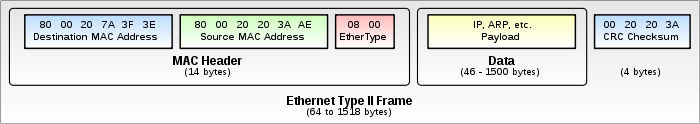
\includegraphics[width=\linewidth]{head_ethernet.png}
	\label{eth}
	\caption{Intestazione protocollo ethernet}
\end{figure}

\newpage
\subsection{Considerazioni input client}
Osservando il grafico in \textit{figura 8.a}, che rappresenta i numeri di sequenza dei pacchetti dal lato client, notiamo come il client invii dati al server. Ciò avviene in 2 casi, quando viene premuto ctrl+C e quando si esce dalla command-mode premendo invio.
Da ciò possiamo evincere che il client invierà dati relativi agli input da tastiera al server.\\
Ciò può essere notato anche nel grafico del payload (\textit{figura 8.b}) dove notiamo la presenza di 2 pacchetti con campo data non nullo (in corrispondenza degli input prima citati).\\
Inoltre da tale grafico si evince che nell'intervallo 7 vi sarà un ritardo tra la pressione del tasto invio e la riapertura della finestra.\\
Notare che nel grafico non si osserva alcun pacchetto relativo all'input da tastiera relativo alla chiusura della connessione nell'ultima command-mode.
S'ipotizza che ciò avvenga in quanto la connessione venga chiusa prima che possano essere inviate informazioni relative a quest'ultimo input.

\begin{figure}[H]
	\begin{subfigure}[l]{0.45\linewidth}
		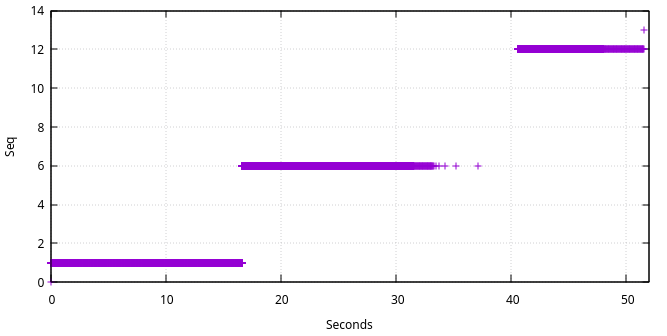
\includegraphics[width=\linewidth]{client_seq_point.png}
		\caption{Seq lato client}
	\end{subfigure}	
	\begin{subfigure}[r]{0.55\linewidth}
		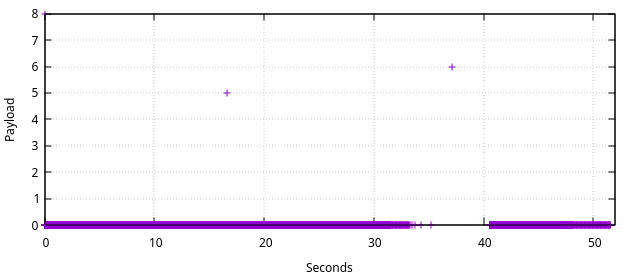
\includegraphics[width=\linewidth]{client_pay_point.png}
		\caption{Pay lato client}
	\end{subfigure}
	\caption{}
\end{figure}
\newpage
\subsection{Script utilizzati}
I file utilizzati per disegnare i grafici sono stati divisi tra client e server.
\subsubsection{Bash}
I file "client.sh" e "server.sh" una volta eseguiti permettono di dividere le colonne dei file "client" e "server" (estratti da wireshark) in piu file,
per poi essere uniti nei files "client.dat" e "server.dat", i quali conterranno i dati utili senza l'intestazione di wireshark (riportata di seguito).

\begin{verbatim}
No.Time Source Destination Protocol Length Seq Info
\end{verbatim}

\begin{lstlisting}
#!/bin/bash
#client.sh
#notare nel calcolo del payload un if in quanto si osserva
#che non tutti i pacchetti hanno stesso numero di byte dedicati alle opzioni.
if [ -e "client.pay" ]; then
    rm client.pay
fi

echo 0 > client.ack #aggiunge Ack alla seconda riga

cat client|tail -n+2|head -1|tr -s " "|cut -d "=" -f 3|\
cut -d " " -f 1 > client.win #prende Win da seconda riga

cat client|tail -n+2|tr -s " "|cut -d " " -f 3 > client.time 
#parte da seconda riga

cat client|tail -n+2|tr -s " "|cut -d " " -f 8 > client.seqn 
#parte da seconda riga

cat client|tail -n+2|grep Ack |tr -s " "|cut -d "=" -f 3|\
cut -d " " -f 1 >> client.ack #parte da terza riga 

cat client|tail -n+3|tr -s " "|cut -d "=" -f 4| cut -d " " -f 1 >> client.win 
#parte da terza riga

cat client|tail -n+2|tr -s " "|cut -d " " -f 7 > tmp
cat tmp | while read line; do
	if [ $line -eq 78 ]; then 
        #nel caso in cui i pacchetti TCP abbiano 24 byte di opzioni
        let x=line-20-44-14 # 4 byte vengono scartati a livello ethernet
    else 
        #nel caso in cui i pacchetti TCP abbiano 12 byte di opzioni
        let x=line-20-32-14 # 4 byte vengono scartati a livello ethernet
    fi
    
    echo $x >>client.pay
done
rm tmp
paste client.time client.seqn client.ack client.win client.pay|\
tr -s " "  > client.dat
\end{lstlisting}
\begin{lstlisting}
#!/bin/bash
#server.sh
if [ -e "server.pay" ]; then
    rm server.pay
fi

cat server | tail -n+2 | tr -s " " | cut -d " " -f 3 > server.time 
#parte da seconda riga

cat server | tail -n+2 | tr -s " " | cut -d " " -f 8 > server.seqn 
#parte da seconda riga

cat server | tail -n+2 | grep Ack  | tr -s " " | cut -d "=" -f 3|\
cut -d " " -f 1 > server.ack #parte da seconda riga 

cat server | tail -n+2 | tr -s " " | cut -d "=" -f 4|\
cut -d " " -f 1 > server.win #parte da seconda riga

cat server | tail -n+2 | tr -s " " | cut -d " " -f 7 > tmp
cat tmp | while read line; do
    let x=line-20-32-14 
    #4 byte vengono scartati a livello ethernet
    echo $x >>server.pay
done
rm tmp
paste server.time server.seqn server.ack server.win server.pay|\
tr -s " "  > server.dat

\end{lstlisting}

\subsubsection{Gnuplot}
Ognuno di questi files specifica nel nome, la sorgente (client o server), un campo di cui osservarne l'evoluzione nel tempo (ACK, WIN ...) e il metodo di visualizzazione del grafico (lines o points).
Tali script possono essere eseguiti con il software GnuPlot utilizzando il comando: \textbf{load "[NOMEFILE]"}.
Di seguito sono elencati i files utili a generare i grafici con interpolazione tra i punti (lines), per ottenere quelli con i soli punti è sufficente eliminare la dicitura with lines al fondo dell'ultima linea\\
\begin{lstlisting}
#plot_client_ACKlines.p
set autoscale
unset log
unset label
set xtic auto
set ytic auto
set title "Client ACK"
set xlabel "Seconds"
set ylabel "Ack"
unset key
set xr [0.0:52.0]
plot "../client.dat" using 1:3 title "Ack(s)" with lines
\end{lstlisting}

\newpage

\begin{lstlisting}
#plot_client_WINlines.p
set autoscale
unset log
unset label
set xtic auto
set ytic auto
set title "Client WIN"
set xlabel "Seconds"
set ylabel "Win size"
unset key
set xr [0.0:52.0]
plot "../client.dat" using 1:4 title "Win(s)" with lines
\end{lstlisting}

\begin{lstlisting}
#plot_client_SEQlines.p
set autoscale
unset log
unset label
set xtic auto
set ytic auto
set title "Client SEQ"
set xlabel "Seconds"
set ylabel "Seq"
unset key
set xr [0.0:52.0]
plot "../client.dat" using 1:2 title "Ack(s)" with lines
\end{lstlisting}



\begin{lstlisting}
#plot_client_PAYlines.p
set autoscale
unset log
unset label
set xtic auto
set ytic auto
set title "Client PAY"
set xlabel "Seconds"
set ylabel "Payload"
unset key
set xr [0.0:52.0]
plot "../client.dat" using 1:5 title "Payload(s)" with lines
\end{lstlisting}

\begin{lstlisting}
#plot_server_ACKlines.p
set autoscale
unset log
unset label
set xtic auto
set ytic auto
set title "Server ACK"
set xlabel "Seconds"
set ylabel "Ack"
unset key
set xr [0.0:52.0]
plot "../server.dat" using 1:3 title "Ack(s)" with lines
\end{lstlisting}

\newpage

\begin{lstlisting}
#plot_server_WINlines.p
set autoscale
unset log
unset label
set xtic auto
set ytic auto
set title "Server WIN"
set xlabel "Seconds"
set ylabel "Win size"
unset key
set xr [0.0:52.0]
plot "../server.dat" using 1:4 title "Win(s)" with lines
\end{lstlisting}

\begin{lstlisting}
#plot_server_SEQlines.p
set autoscale
unset log
unset label
set xtic auto
set ytic auto
set title "Server SEQ"
set xlabel "Seconds"
set ylabel "Seq"
unset key
set xr [0.0:52.0]
plot "../server.dat" using 1:2 title "Seq(s)" with lines
\end{lstlisting}


\begin{lstlisting}
#plot_server_PAYlines.p
set autoscale
unset log
unset label
set xtic auto
set ytic auto
set title "Server PAY"
set xlabel "Seconds"
set ylabel "Payload"
unset key
set xr [0.0:52.0]
plot "../server.dat" using 1:5 title "Payload(s)" with lines
\end{lstlisting}

\newpage
\subsection{Grafici}
Di seguito sono stati inseriti i grafici richiesti e non presenti nel resto della realazione
\subsubsection{Client}
\begin{figure}[H]
	\center
	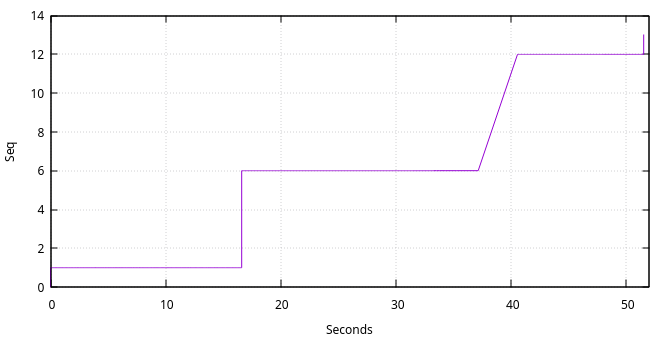
\includegraphics[width=0.75\linewidth]{client_seq_lines.png}
	\label{eth}
	\caption{Seq lato client}
\end{figure}

\begin{figure}[H]
	\center
	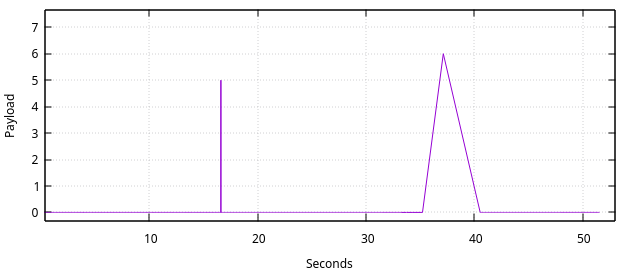
\includegraphics[width=0.75\linewidth]{client_pay_lines.png}
	\label{eth}
	\caption{Pay lato client}
\end{figure}

\begin{figure}[H]
	\center
	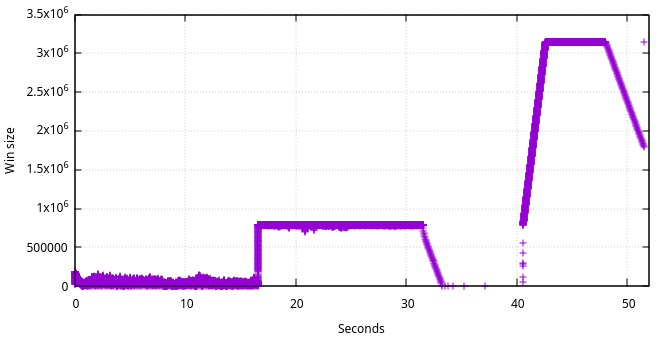
\includegraphics[width=0.75\linewidth]{client_win_point.png}
	\label{eth}
	\caption{Win lato client (no interpolazione)}
\end{figure}

\subsubsection{Server}
\begin{figure}[H]
	\center
	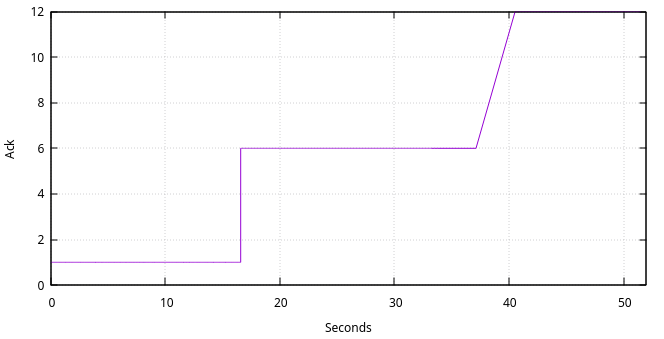
\includegraphics[width=0.75\linewidth]{server_ack_lines.png}
	\label{eth}
	\caption{Ack lato server}
\end{figure}

\begin{figure}[H]
	\center
	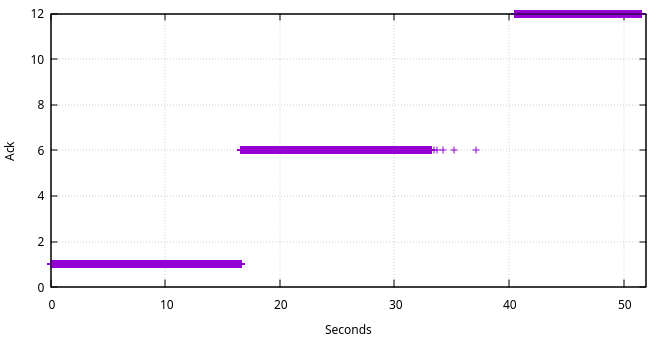
\includegraphics[width=0.75\linewidth]{server_ack_point.png}
	\label{eth}
	\caption{Ack lato server (no interpolazione)}
\end{figure}

\begin{figure}[H]
	\center
	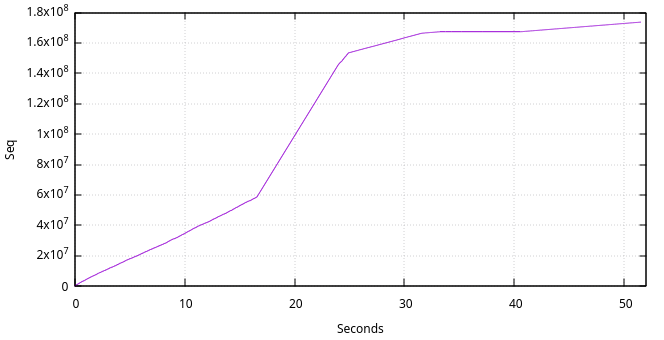
\includegraphics[width=0.75\linewidth]{server_seq_lines.png}
	\label{eth}
	\caption{Seq lato server}
\end{figure}

\begin{figure}[H]
	\center
	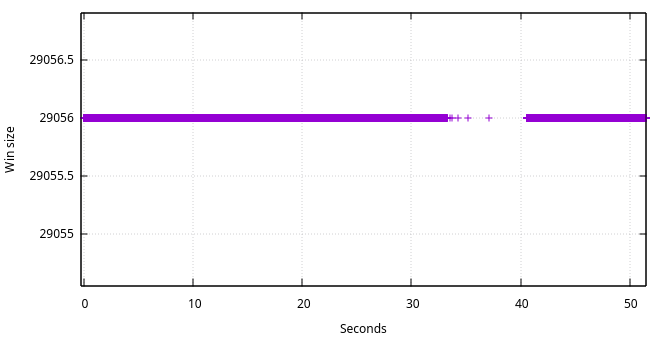
\includegraphics[width=0.75\linewidth]{server_win_point.png}
	\label{eth}
	\caption{Win lato server (no interpolazione)}
\end{figure}

\begin{figure}[H]
	\center
	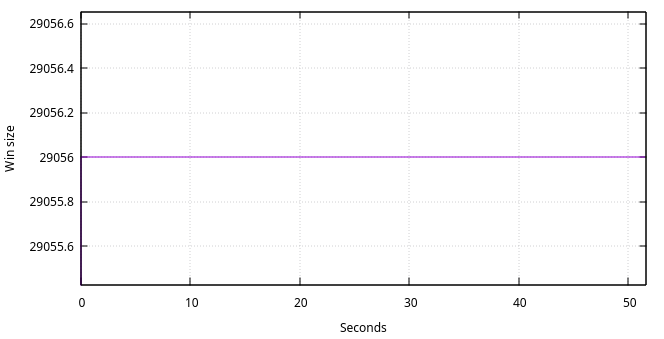
\includegraphics[width=0.75\linewidth]	{server_win_lines.png}
	\label{eth}
	\caption{Win lato server}
\end{figure}

\begin{figure}[H]
	\center
	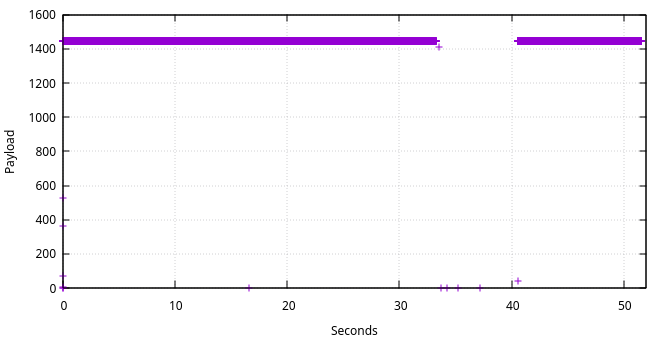
\includegraphics[width=0.75\linewidth]{server_pay_points.png}
	\label{eth}
	\caption{Pay lato server (no interpolazione)}
\end{figure}

\begin{figure}[H]
	\center
	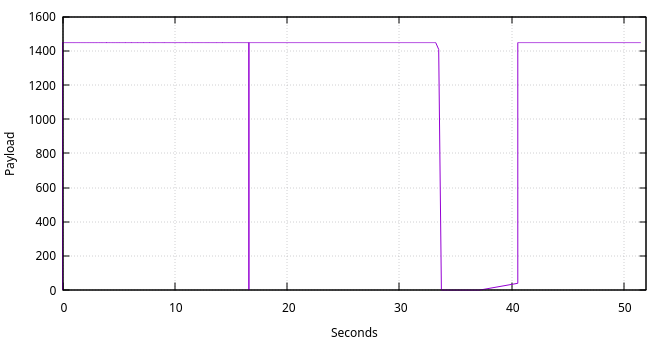
\includegraphics[width=0.75\linewidth]{server_pay_lines.png}
	\label{eth}
	\caption{Pay lato server}
\end{figure}

\end{document}
